%

\subsection{Evaluation on Image Captioning}
\subsubsection{Dataset}
%
We report image captioning results on the popular Flickr8k \cite{hodosh2013framing}, Flickr30k \cite{young2014image} and Microsoft COCO dataset \cite{lin2014microsoft}. These datasets contain 8,000, 31,000 and 123,287 images respectively, and each image is annotated with 5 sentences. In our reported results, we use pre-defined splits for Flickr8k.%
Because most of previous works in image captioning \cite{donahue2014long,fang2014captions,Karpathy2014deepvs,mao2014deep,vinyals2014show,xu2015show} are not evaluated on the official split for Flickr30k and MS COCO, for fair comparison, we report results with the widely used publicly available splits in the work of \cite{Karpathy2014deepvs}.%
We further tested on the actually MS COCO test set consisting of 40775 images (human captions for this split are not available publicly), and evaluated them on the COCO evaluation server.

\begin{table}[t]
\begin{center}
\scriptsize
\resizebox{1\linewidth}{!}{
 \begin{tabular}{ l c c c c|c }
    %
    \multicolumn{6}{c}{Flickr8k}\\
    \Xhline{2\arrayrulewidth}
    \textbf{State-of-art-Flickr8k} & B-1 & B-2 & B-3 & B-4 & $\mathcal{PPL}$ \\ \hline
    Karpathy \& Li (NeuralTalk) \cite{Karpathy2014deepvs}& 0.58 & 0.38 & 0.25 & 0.16 & - \\
    Chen \& Zintick (Mind's Eye) \cite{Chen2015CVPRMind}&-&-&-&0.14&15.10 \\
    Google(NIC)\cite{vinyals2014show}& 0.66 & 0.42 & 0.27 &0.18&- \\
    Mao et al. (m-Rnn-AlexNet) \cite{mao2014deep}&0.57&0.39&0.26&0.17&24.39 \\
    Xu et al. (Hard-Attention) \cite{xu2015show}&0.67&0.46&0.31&0.21&- \\
    \Xhline{2\arrayrulewidth}
    \textbf{Baseline - \textit{CNN(I)}} & & & & & \\ \hline
    VggNet+LSTM & 0.56 & 0.37 & 0.24 & 0.16 & 15.71 \\
    VggNet-PCA+LSTM & 0.56 & 0.38 & 0.25 & 0.16 &16.07 \\
    %
    VggNet+ft+LSTM & 0.64 & 0.43 & 0.30 & 0.20 & 14.69 \\
    \Xhline{2\arrayrulewidth}
    \textbf{Ours - $\Att(I)$} & & & & & \\ \hline
    %
    \cellcolor[rgb]{0.7,0.7,0.7}{Att-GT+LSTM\textsuperscript{$\ddagger$}} & \cellcolor[rgb]{0.7,0.7,0.7}{0.76} & \cellcolor[rgb]{0.7,0.7,0.7}{0.57} & \cellcolor[rgb]{0.7,0.7,0.7}{0.41} & \cellcolor[rgb]{0.7,0.7,0.7}{0.29} & \cellcolor[rgb]{0.7,0.7,0.7}{12.52}\\
    %
    Att-SVM+LSTM & 0.73 & 0.53 & \textbf{0.38} & 0.26 & 12.63\\
    Att-GlobalCNN+LSTM&0.72&0.53&\textbf{0.38}&\textbf{0.27}&12.63\\
    Att-RegionCNN+LSTM & \textbf{0.74} & \textbf{0.54} & \textbf{0.38} & \textbf{0.27} & \textbf{12.60}\\
    \Xhline{2\arrayrulewidth}
    \vspace{1pt}
 \end{tabular}}
 \scriptsize
 \resizebox{1\linewidth}{!}{
 \begin{tabular}{l c c c c|c }
    %
    \multicolumn{6}{c}{Flickr30k}\\
    \Xhline{2\arrayrulewidth}
    \textbf{State-of-art-Flickr30k} & B-1 & B-2 & B-3 & B-4 & $\mathcal{PPL}$ \\ \hline
    Karpathy \& Li (NeuralTalk) \cite{Karpathy2014deepvs}& 0.57 & 0.37 & 0.24 & 0.16 & - \\
    Chen \& Zintick (Mind's Eye) \cite{Chen2015CVPRMind}& -&-&-&0.13&19.10 \\
    Google(NIC) \cite{vinyals2014show}& 0.66 & - & - &-&- \\
    Donahue et al. (LRCN) \cite{donahue2014long}&0.59&0.39&0.25&0.17&- \\
    Mao et al. (m-Rnn-AlexNet) \cite{mao2014deep}&0.54&0.36&0.23&0.15&35.11 \\
    Mao et al. (m-Rnn-VggNet) \cite{mao2014deep}&0.60&0.41&0.28&0.19&20.72 \\
    Xu et al. (Hard-Attention) \cite{xu2015show}&0.67&0.44&0.30&0.20&- \\
    \Xhline{2\arrayrulewidth}
    \textbf{Baseline - \textit{CNN(I)}} & & & & & \\ \hline
    VggNet+LSTM & 0.57 & 0.38 & 0.25 & 0.17 & 18.83 \\
    VggNet-PCA+LSTM & 0.59 & 0.40 & 0.26 & 0.17 & 18.92 \\
    %
    VggNet+ft+LSTM & 0.67 & 0.47 & 0.31 & 0.21 & 16.62 \\\Xhline{2\arrayrulewidth}
    \textbf{Ours - $\Att(I)$} & & & & & \\ \hline
    %
    \cellcolor[rgb]{0.7,0.7,0.7}{Att-GT+LSTM\textsuperscript{$\ddagger$}} & \cellcolor[rgb]{0.7,0.7,0.7}{0.78} & \cellcolor[rgb]{0.7,0.7,0.7}{0.57} & \cellcolor[rgb]{0.7,0.7,0.7}{0.42} & \cellcolor[rgb]{0.7,0.7,0.7}{0.30} & \cellcolor[rgb]{0.7,0.7,0.7}{14.88} \\
    %
    Att-SVM+LSTM & 0.68 & 0.49 & 0.33 &0.23 & 16.01 \\
    Att-GlobalCNN+LSTM&0.70&0.50&0.35&0.27&16.00\\
    Att-RegionCNN+LSTM & \textbf{0.73} & \textbf{0.55} & \textbf{0.40} & \textbf{0.28} & \textbf{15.96}\\
    \Xhline{2\arrayrulewidth}
  \end{tabular}}
\end{center}
  \vspace{-5pt}
 \caption{BLEU-1,2,3,4 and $\mathcal{PPL}$ metrics compared to other state-of-the-art methods and our baseline on Flickr8k and Flickr30K dataset. $\ddagger$~indicates ground truth attributes labels are used, which (in \colorbox[rgb]{0.7,0.7,0.7}{gray}) will not participate in rankings. Our $\mathcal{PPL}s$ are based on Flickr8k and Flickr30k word dictionaries of size 2538 and 7414, respectively.}
 \vspace{-10pt}
\label{tab1} 
\end{table}

\subsubsection{Evaluation}
\textbf{Metrics:}
We report results with the frequently used BLEU metric \cite{papineni2002bleu} and sentence perplexity ($\mathcal{PPL}$). %
For MS COCO dataset, we additionally evaluate our model based on the metrics of METEOR \cite{banerjee2005meteor} and CIDEr \cite{vedantam2014cider}. %

\begin{table}[t]
\begin{center}
\scriptsize
  \resizebox{1\linewidth}{!}{%
  \begin{tabular}{ l c c c c c c|c}
    \Xhline{2\arrayrulewidth}
    \textbf{State-of-art} &B-1 & B-2 & B-3 & B-4 & M & C & $\mathcal{P}$ \\ \hline
    NeuralTalk \cite{Karpathy2014deepvs}& 0.63 & 0.45 & 0.32 & 0.23 & 0.20& 0.66&- \\
    Mind's Eye \cite{Chen2015CVPRMind}& -&-&-&0.19&0.20&-&11.60 \\
    NIC \cite{vinyals2014show}& - & - & - &0.28&0.24&0.86&- \\
    LRCN \cite{donahue2014long}&0.67&0.49&0.35&0.25&-&-&- \\
    Mao et al.\cite{mao2014deep}&0.67&0.49&0.34&0.24&-&-&13.60 \\
    %
    Jia et al.\cite{jia2015guilding}&0.67&0.49&0.36&0.26&0.23&0.81&- \\
    MSR \cite{fang2014captions}&-&-&-&0.26&0.24&-&18.10\\
    Xu et al.\cite{xu2015show}&0.72&0.50&0.36&0.25&0.23&-&- \\
    Jin et al.\cite{jin2015aligning}&0.70&0.52&0.38&0.28&0.24&0.84&- \\
    \Xhline{2\arrayrulewidth}
    \textbf{Baseline-\textit{CNN(I)}} &  &  &  & & & & \\ \hline
    VNet+LSTM & 0.61 & 0.42 & 0.28 & 0.19 &0.19 &0.56&13.58  \\
    VNet-PCA+LSTM & 0.62 & 0.43 & 0.29 & 0.19 &0.20 &0.60&13.02 \\
    %
    VNet+ft+LSTM & 0.68 & 0.50 & 0.37 & 0.25 & 0.22&0.73& 13.29 \\
    \Xhline{2\arrayrulewidth}
    \textbf{Ours-$\Att(I)$} & & & & & &&\\ \hline
    %
    \cellcolor[rgb]{0.7,0.7,0.7}{Att-GT+LSTM\textsuperscript{$\ddagger$}} & \cellcolor[rgb]{0.7,0.7,0.7}{0.80} & \cellcolor[rgb]{0.7,0.7,0.7}{0.64} & \cellcolor[rgb]{0.7,0.7,0.7}{0.50} & \cellcolor[rgb]{0.7,0.7,0.7}{0.40} &\cellcolor[rgb]{0.7,0.7,0.7}{0.28} & \cellcolor[rgb]{0.7,0.7,0.7}{1.07}&\cellcolor[rgb]{0.7,0.7,0.7}{9.60} \\
    %
    Att-SVM+LSTM & 0.69 & 0.52 & 0.38  &0.28 & 0.23& 0.82&12.62  \\
    %
    %
    %
    %
    Att-GlobalCNN+LSTM & 0.72  & 0.54  & 0.40   &0.30  & 0.25 & 0.83 &11.39    \\
    Att-RegionCNN+LSTM & \textbf{0.74} & \textbf{0.56} & \textbf{0.42}  & \textbf{0.31} & \textbf{0.26}& \textbf{0.94}& \textbf{10.49} \\ \hline
    %
    %
    %
  \end{tabular}}
      \vspace{-4pt}
      \caption{BLEU-1,2,3,4, METEOR, CIDEr and $\mathcal{PPL}$ metrics compared to other state-of-the-art methods and our baseline on MS COCO dataset. $\ddagger$~indicates ground truth attributes labels are used, which (in \colorbox[rgb]{0.7,0.7,0.7}{gray}) will not participate in rankings. Our $\mathcal{PPL}s$ are based on MS COCO word dictionaries of size 8791.}
      \label{tab2}
      \vspace{-25pt}
\end{center}
\end{table}

\vspace{3pt}
\noindent\textbf{Baselines:}
To verify the effectiveness of our high-level attributes representation, we provide a baseline method. The baseline framework is same as the one proposed in section \ref{subsec:caption_model}, except that the attributes vector $\Att(I)$ is replaced by the last hidden layer of CNN directly. %
For the \textbf{VggNet+LSTM}, we use the second fully connected layer (\texttt{fc7}) as the image features, which has 4096 dimensions. In \textbf{VggNet-PCA+LSTM}, PCA is applied to decrease the feature dimension from 4096 to 1000. %
\textbf{VggNet+ft+LSTM} applies a VggNet that has been fine-tuned on the target dataset, based on the task of image-attributes classification.

\vspace{3pt}
\noindent\textbf{Our Approaches:}
We evaluate several variants of our approach: \textbf{Att-GT+LSTM} models use ground-truth attributes as the input while \textbf{Att-RegionCNN+LSTM} uses the attributes vector $\Att(I)$ predicted by the region based attributes prediction network in section \ref{subsec:Attributes_Predictor}. We also evaluate an approach \textbf{Att-SVM+LSTM} with linear SVM predicted attributes vector. %
We use the second fully connected layer of the fine-tuned VggNet to feed the SVM. To verify the effectiveness of the region based attributes prediction in the captioning task, the \textbf{Att-GlobalCNN+LSTM} is implemented by using the global image for attributes prediction.

\vspace{3pt}
\noindent\textbf{Results:} Table \ref{tab1} and \ref{tab2} report image captioning results on Flickr8k, Flickr30k and Microsoft COCO dataset. It is not surprising that \textbf{Att-GT+LSTM} model performs best, since ground truth attributes labels are used. We report these results here just to show the advances of adding an intermediate image-to-word mapping stage. Ideally, if we could train a perfectly accurate attribute predictor, we could obtain an outstanding improvement compared to both baseline and state-of-the-art methods. Indeed, apart from using ground truth attributes, our \textbf{Att-RegionCNN+LSTM} models generate the best results on all the three datasets over all evaluation metrics. Especially comparing with baselines, which do not contain an attributes prediction layer, our final models bring significant improvements, nearly 15\% for B-1 and 30\% for CIDEr on average. \textbf{VggNet+ft+LSTM} models perform better than other baselines because of the fine-tuning on the target dataset. However, they do not perform as well as our attributes-based models. \textbf{Att-SVM+LSTM} and \textbf{Att-GlobalCNN+LSTM} under-perform \textbf{Att-RegionCNN+LSTM}, indicating that region-based attributes prediction provides useful detail beyond whole image classification. Our final model also outperforms the current state-of-the-art listed in the tables. We also evaluated an approach (not shown in table) that combines CNN features and attributes vector together as the input of the LSTM, but we found this approach is not as good as using attributes vector only in the same setting.  In any case, above experiments show that an intermediate image-to-words stage (i.e. attributes prediction layer) bring us significant improvements.

\begin{table}[t!]
\begin{center}
\scriptsize
\resizebox{\linewidth}{!}{
  \begin{tabular}{ l c c c c c c c }
    \Xhline{2\arrayrulewidth}
    COCO-TEST & B-1 & B-2 & B-3&B-4 & M & R &CIDEr\\ \hline
    \textbf{5-Refs} &&&&&&& \\\hline
    Ours&0.73&0.56&0.41&0.31&0.25&0.53&0.92\\
    Human&0.66&0.47&0.32&0.22&0.2&0.48&0.85\\
    MSR \cite{fang2014captions}&0.70&0.53&0.39&0.29&0.25&0.52&0.91\\
    m-RNN \cite{mao2014deep}&0.68&0.51&0.37&0.27&0.23&0.50&0.79\\
    LRCN \cite{donahue2014long}&0.70&0.53&0.38&0.28&0.24&0.52&0.87\\
    Montreal \cite{xu2015show}&0.71&0.53&0.38&0.28&0.24&0.52&0.87\\
    Google \cite{vinyals2014show}&0.71&0.54&0.41&0.31&0.25&0.53&0.94\\
    NeuralTalk\cite{Karpathy2014deepvs}&0.65&0.46&0.32&0.22&0.21&0.48&0.67\\
    MSR Captivator\cite{devlin2015language}&0.72&0.54&0.41&0.31&0.25&0.53&0.93\\
    Nearest Neighbor \cite{devlin2015exploring}&0.70&0.52&0.38&0.28&0.24&0.51&0.89\\
    MLBL \cite{kiros2014multimodal}&0.67&0.50&0.36&0.26&0.22&0.50&0.74\\
    ATT \cite{you2016image}&0.73&0.57&0.42&0.32&0.25&0.54&0.94\\
    \Xhline{2\arrayrulewidth}
    \textbf{40-Refs} &&&&&&& \\\hline
    Ours&0.89&0.80&0.69&0.58&0.33&0.67&0.93\\
    Human&0.88&0.74&0.63&0.47&0.34&0.63&0.91\\
    MSR \cite{fang2014captions}&0.88&0.79&0.68&0.57&0.33&0.66&0.93\\
    m-RNN \cite{mao2014deep}&0.87&0.76&0.64&0.53&0.30&0.64&0.79\\
    LRCN \cite{donahue2014long}&0.87&0.77&0.65&0.53&0.32&0.66&0.89\\
    Montreal \cite{xu2015show}&0.88&0.78&0.66&0.54&0.32&0.65&0.89\\
    Google \cite{vinyals2014show}&0.89&0.80&0.69&0.59&0.35&0.68&0.95\\
    NeuralTalk\cite{Karpathy2014deepvs}&0.83&0.70&0.57&0.45&0.28&0.60&0.69\\
    MSR Captivator\cite{devlin2015language}&0.90&0.82&0.71&0.60&0.34&0.68&0.94\\
    Nearest Neighbor \cite{devlin2015exploring}&0.87&0.77&0.66&0.54&0.32&0.65&0.92\\
    MLBL \cite{kiros2014multimodal}&0.85&0.75&0.63&0.52&0.29&0.64&0.75\\
    ATT \cite{you2016image}&0.90&0.82&0.71&0.60&0.34&0.68&0.96\\
    \Xhline{2\arrayrulewidth}
  \end{tabular}}
  \vspace{-4pt}
  \caption{COCO evaluation server results. M and R stands for METEOR and ROUGE-L.
  Results using 5 references and 40 references captions are both shown. We only list the comparison results that have been officially published in the corresponding references. Please note some of them are concurrent results with this submission, such as \cite{you2016image}.}
  \label{tab3}
  \vspace{-23pt}
\end{center}
\end{table}

We further generated captions for the images in the COCO test set containing 40,775 images and evaluated them on the COCO evaluation server. These results are shown in Table \ref{tab3}. We achieve 0.73 on B-1, and surpass human performances on 13 of the 14 metrics reported. Other state-of-the-art methods are also shown for comparison.

\noindent\textbf{Human Evaluation:} We additionally perform a human evaluation on our proposed model, to evaluate the caption generation ability. We randomly sample 1000 results from the COCO validation dataset, generated by our proposed model Att-RegionCNN+LSTM and the baseline model VggNet+LSTM. Following the human evaluation protocol of the MS COCO Captioning Challenge 2015, two evaluation metrics are applied. M1 is the percentage of captions that are evaluated as better or equal to human caption and M2 is the percentage of captions that pass the Turing Test. Table \ref{tab_human} summarizes the human evaluation results. We can see our model outperforms the baseline model on both metrics. We did not evaluate on the test split because the human ground truth is not publicly available.

\begin{table}[h!]
\begin{center}
\vspace{-5pt}
\resizebox{\linewidth}{!}{
  \begin{tabular}{ >{\centering\arraybackslash}m{4cm} >{\centering\arraybackslash}m{2cm} >{\centering\arraybackslash}m{2cm} }
    \Xhline{2\arrayrulewidth}
     & Ours & VggNet+LSTM\\ \hline
    M1: percentage of captions that are evaluated as better or equal to human caption. &0.25&0.15\\ \hline
    M2: percentage of captions that pass the Turing Test. &0.30&0.19\\
    \Xhline{2\arrayrulewidth}
  \end{tabular}}
  \vspace{-3pt}
  \caption{ Human Evaluation on 1000 sampled results from MS COCO validation split.
  }
  \vspace{-20pt}
  \label{tab_human}
\end{center}
\end{table}

\begin{table}[t!]
\begin{center}
\scriptsize
\resizebox{\linewidth}{!}{
  \begin{tabular}{ c c c c c c}
    \Xhline{2\arrayrulewidth}
      & Ours & NIC\cite{vinyals2014show} & LRCN\cite{donahue2014long} & m-RNN\cite{mao2014deep} & NeuralTalk\cite{Karpathy2014deepvs}\\ \hline
    VIS Input Dim&256&1000&1000&4096&4096\\
    RNN Dim&256&512&1000$\times2/4$&256&300-600\\
    \Xhline{2\arrayrulewidth}
  \end{tabular}}
  \vspace{-3pt}
  \caption{Visual feature input dimension and properties of RNN. Our visual features has been encoded as a 256-d attributes score vector while other models need higher dimensional features to feed to RNN. According to the unit size of RNN, we achieve state-of-the-art using a relatively small dimensional recurrent layer. 
  }
  \vspace{-15pt}
  \label{tab3-2}
\end{center}
\end{table}

Table \ref{tab3-2} summarizes some properties of recurrent layers employed in some recent RNN-based methods.  We achieve state-of-the-art using a relatively low dimensional visual input feature and recurrent layer. Lower dimension of visual input and RNN normally means less parameters in the RNN training stage, as well as lower computation cost.

\subsection{Evaluation on Visual Question Answering}
We evaluate our model on four recent publicly available visual question answering datasets.
DAQURA-ALL is proposed in \cite{malinowski2014towards}. There are 7,795 training questions and 5,673 test questions. %
DAQURA-REDUCED is a reduced version of DAQURA-ALL. There are 3,876 training questions and only 297 test questions. This dataset is constrained to 37 object categories and uses only 25 test images. Two large-scale VQA data are constructed both based on MS COCO images. The Toronto COCO-QA Dataset \cite{ren2015image} contains 78,736 training and 38,948 testing examples, which are generated from 117,684 images. %
All of the question-answer pairs in this dataset are automatically converted from human-sourced image descriptions. Another benchmarked dataset is VQA~\cite{antol2015vqa}, which is a much larger dataset and contains 614,163 questions and 6,141,630 answers based on 204,721 MS COCO images. %
We randomly choose 5000 images from the validation set as our val set, with the remainder testing. The human ground truth answers for the actual VQA test split are not available publicly and only can be evaluated via the VQA evaluation server. Hence, we also apply our final model on a test split and report the overall accuracy. Table \ref{tab:data} displays some dataset statistics. %

\begin{table}[h]
\begin{center}
\scriptsize
\resizebox{\linewidth}{!}{
 \begin{tabular}{l c c c c}
 \Xhline{2\arrayrulewidth}
 &DAQURA&DAQURA&Toronto& \\ 
 &All&Reduced&COCO-QA&VQA \\\hline
 \# Images&1,449&1,423&117,684&204,721 \\
 \# Questions&12,468&4,173&117,684&614,163 \\
 \# Question Types&3&3&4&more than 20 \\
 \# Ans per Que&1&1&1&10\\
 \# Words per Ans&1+&1+&1&1+\\ \Xhline{2\arrayrulewidth}
 \end{tabular}}
 \vspace{-3pt}
 \caption{Some statistics about the DAQURA, Toronto COCO-QA Dataset \cite{ren2015image} and VQA dataset~\cite{antol2015vqa}.}
 \label{tab:data}
 %
\end{center}
\end{table}

\subsubsection{Results on DAQURA}
\textbf{Metrics:}
Following \cite{ma2015learning, ren2015image}, the accuracy value (the proportion of correctly answered test questions), and the Wu-Palmer similarity (WUPS) \cite{wu1994verbs} are used to measure performance. The WUPS calculates the similarity between two words based on the similarity between their common subsequence in the taxonomy tree. If the similarity between two words is greater than a threshold then the candidate answer is considered to be right. We report on thresholds 0.9 and 0.0, following~\cite{ma2015learning,ren2015image}.

\vspace{3pt}
\noindent\textbf{Evaluations:}
To illustrate the effectiveness of our model, we provide two baseline models and several state-of-the-art results in table \ref{tab:DAQURA_All} and \ref{tab:DAQURA-Reduced}. The \textbf{Baseline} method is implemented simply by connecting a CNN to an LSTM. The CNN is a pre-trained (on ImageNet) VggNet model from which we extract the coefficients of the last fully connected layer. We also implement a baseline model \textbf{VggNet+ft-LSTM}, which applies a vggNet that has been fine-tuned on the COCO dataset, based on the task of image-attributes classification. We also present results from a series of cut down versions of our approach for comparison. \textbf{Att-LSTM} uses only the semantic level attribute representation $\Att$ as the LSTM input. To evaluate the contribution of the internal textual representation and external knowledge for the question answering, we feed the image caption representation $\Cap$ and knowledge representation $\Know$ with the $\Att$ separately, producing two models, \textbf{Att+Cap-LSTM} and \textbf{Att+Know-LSTM}. We also tested the \textbf{Cap+Know-LSTM}, for the experiment completeness. \textbf{Att+Cap+Know-LSTM} combines all the available information. Our final model is the \textbf{A+C+Selected-K-LSTM}, which uses the selected knowledge information (see section \ref{subsec:selected}) as the input. \textbf{GUESS} \cite{ren2015image} simply selects the modal answer from the training set for each of 4 question types.  %
\textbf{VIS+BOW}~\cite{ren2015image} performs multinomial logistic regression based on image features and a BOW vector obtained by summing all the word vectors of the question. \textbf{VIS+LSTM}~\cite{ren2015image} has one LSTM to encode the image and question, while \textbf{2-VIS+BLSTM}~\cite{ren2015image} has two image feature inputs, at the start and the end. Malinowski\etal~\cite{malinowski2015ask} propose a neural-based approach and Ma \textit{et al.}~\cite{ma2015learning} encodes both images and questions with a CNN. Yang~\etal~\cite{yang2015stacked} use a stacked attention networks to infer the answer progressively.

\begin{table}[t!]
\scriptsize
\begin{center}
\resizebox{\linewidth}{!}{
    \begin{tabular}{ l|c c c }
    \Xhline{2\arrayrulewidth}
    \textbf{DAQURA-All} &Acc(\%) & WUPS@0.9 & WUPS@0.0 \\ \hline
    Askneuron\cite{malinowski2015ask}&19.43&25.28&62.00\\
    Ma~\etal\cite{ma2015learning}&23.40&29.59&62.95\\
    Yang~\etal\cite{yang2015stacked}&\textbf{29.30}&35.10&68.60\\
    Noh~\etal\cite{Noh2015image}&28.98&34.80&67.81\\
    \Xhline{2\arrayrulewidth}
    \textbf{Baseline} &  &   &   \\ \hline
    VggNet-LSTM & 23.13 & 30.01 & 63.61 \\
    VggNet+ft-LSTM & 23.75 & 30.22 & 63.66 \\
    Human Baseline\cite{malinowski2015ask} & 50.20 & 50.82 & 62.27 \\
    \Xhline{2\arrayrulewidth}
    \textbf{Our-Proposal} &  &   &   \\ \hline
    Att-LSTM& 24.27& 30.41& 62.29 \\
    Att+Cap-LSTM& 27.04& 33.40& 67.65 \\
    Att+Know-LSTM& 24.89& 31.27& 66.11 \\
    Cap+Know-LSTM& 23.91& 30.64& 65.01 \\
    Att+Cap+Know-LSTM& 29.16& 35.30& 68.66 \\
    A+C+Selected-K-LSTM& 29.23& \textbf{35.37}&\textbf{68.72}\\
    \Xhline{2\arrayrulewidth}
    \end{tabular}}
    \vspace{-3pt}
    \caption{Accuracy, WUPS metrics compared to other state-of-the-art methods and our baseline on DAQURA-All.}
    \label{tab:DAQURA_All}
    \vspace{-8pt}
\end{center}
\end{table}

\begin{table}[t!]
\scriptsize
\begin{center}
\resizebox{\linewidth}{!}{
    \begin{tabular}{ l|c c c }
    \Xhline{2\arrayrulewidth}
    \textbf{DAQURA-Reduced} &Acc(\%) & WUPS@0.9 & WUPS@0.0 \\ \hline
    GUESS\cite{ren2015image}&18.24&29.65&77.59 \\
    VIS+BOW\cite{ren2015image}&34.17&44.99&81.48 \\
    VIS+LSTM\cite{ren2015image}&34.41&46.05&82.23 \\
    2-VIS+BLSTM\cite{ren2015image}&35.78&46.83&82.15 \\
    Askneuron\cite{malinowski2015ask}&34.68&40.76&79.54\\
    Ma~\etal\cite{ma2015learning}&39.66&44.86&83.06\\
    Xu~\etal\cite{xu2015ask}&40.07&-&-\\
    Yang~\etal\cite{yang2015stacked}&45.50&50.20&83.60\\
    Noh~\etal\cite{Noh2015image}&44.48&49.56&\textbf{83.95}\\
    \Xhline{2\arrayrulewidth}
    \textbf{Baseline} &  &   &   \\ \hline
    VggNet-LSTM & 38.72 & 43.97 & 83.01 \\
    VggNet+ft-LSTM & 39.13 & 44.03 & 83.33 \\
    Human Baseline\cite{malinowski2015ask} & 60.27 & 61.04 & 78.96 \\
    \Xhline{2\arrayrulewidth}
    \textbf{Our-Proposal} &  &   &   \\ \hline
    Att-LSTM& 40.07& 45.43& 82.67 \\
    Att+Cap-LSTM&44.78&50.07&83.85\\
    Att+Know-LSTM& 41.08& 46.04& 82.39 \\   
    Cap+Know-LSTM& 40.81& 45.04& 82.01 \\   
    Att+Cap+Know-LSTM& 45.79& 51.53&83.91\\
    A+C+Selected-K-LSTM& \textbf{46.13}& \textbf{51.83}&\textbf{83.95}\\
     \Xhline{2\arrayrulewidth}
    \end{tabular}}
    \vspace{-3pt}
    \caption{Accuracy, WUPS metrics compared to other state-of-the-art methods and our baseline on DAQURA-Reduced.}
    \label{tab:DAQURA-Reduced}
    \vspace{-20pt}
\end{center}
\end{table}

All of our proposed models outperform the \textbf{Baseline} method. And our final model \textbf{A+C+Selected-K-LSTM} achieves the best state-of-the-art on the DAQURA-Reduced set. \textbf{Att+Cap+Know-LSTM} performs not as good as \textbf{A+C+Selected-K-LSTM}, which shows the effectiveness of our question-based knowledge selection scheme.

\subsubsection{Results on Toronto COCO-QA}

\begin{table}[t!]
%
\scriptsize
\begin{center}
\resizebox{\linewidth}{!}{
    \begin{tabular}{ l|c c c }
    \Xhline{2\arrayrulewidth}
    \textbf{Toronto COCO-QA} &Acc(\%) & WUPS@0.9 & WUPS@0.0 \\ \hline
    GUESS\cite{ren2015image}&6.65&17.42&73.44 \\
    VIS+BOW\cite{ren2015image}&55.92&66.78&88.99 \\
    VIS+LSTM\cite{ren2015image}&53.31&63.91&88.25 \\
    2-VIS+BLSTM\cite{ren2015image}&55.09&65.34&88.64 \\
    Ma~\etal\cite{ma2015learning}&54.95&65.36&88.58\\
    Chen~\etal\cite{Chen2015ABC}&58.10&68.44&89.85\\
    Yang~\etal\cite{yang2015stacked}&61.60&71.60&90.90\\
    Noh~\etal\cite{Noh2015image}&61.19&70.84&90.61\\
    \Xhline{2\arrayrulewidth}
    \textbf{Baseline} &  &   &   \\ \hline
    VggNet-LSTM & 50.73 & 60.37 & 87.48 \\
    VggNet+ft-LSTM & 58.34 & 67.32 & 89.13 \\
    \Xhline{2\arrayrulewidth}
    \textbf{Our-Proposal} &  &   &   \\ \hline
    Att-LSTM& 61.38& 71.15& 91.58 \\
    Att+Cap-LSTM& 69.02& 76.20& 92.38 \\
    Att+Know-LSTM& 63.07& 72.22& 90.84 \\
    Cap+Know-LSTM& 64.31& 73.31& 90.01 \\
    Att+Cap+Know-LSTM& 69.73& 77.14& 92.50 \\
    A+C+Selected-K-LSTM& \textbf{70.98}& \textbf{78.35}& \textbf{92.87} \\
     \Xhline{2\arrayrulewidth}
    \end{tabular}}
    \vspace{-3pt}
    \caption{Accuracy, WUPS metrics compared to other state-of-the-art methods and our baseline on Toronto COCO-QA dataset.}
    \label{tab:coco_QA}
    \vspace{-7pt}
\end{center}
\end{table}

\vspace{3pt}
\noindent\textbf{Evaluations:}
%
%
\begin{table}[t!]
%
\scriptsize
%
\resizebox{\linewidth}{!}{
    \begin{tabular}{ l|c c c c }
    \Xhline{2\arrayrulewidth}
    \textbf{Toronto COCO-QA} &Object & Number & Color & Location \\ \hline
    GUESS\cite{ren2015image}&2.11&35.84&13.87& 8.93\\
    VIS+BOW\cite{ren2015image}&58.66&44.10&51.96&49.39 \\
    VIS+LSTM\cite{ren2015image}&56.53&46.10&45.87&45.52 \\
    2-VIS+BLSTM\cite{ren2015image}&58.17&44.79&49.53&47.34 \\
    Chen~\etal\cite{Chen2015ABC}&62.46&45.70&46.81&53.67\\
    Yang~\etal\cite{yang2015stacked}&64.50&48.60&57.90&54.00\\
    %
    \Xhline{2\arrayrulewidth}
    \textbf{Baseline} & &   & &  \\ \hline
    VggNet-LSTM &53.71&45.37&36.23&46.37 \\
    VggNet+ft-LSTM &61.67&50.04&52.16&54.40 \\
    \Xhline{2\arrayrulewidth}
    \textbf{Our-Proposal} &  &   & &  \\ \hline
    Att-LSTM&63.92&51.83&57.29&54.84 \\
    Att+Cap-LSTM&71.30&69.98&61.50&60.98 \\
    Att+Know-LSTM&64.57&54.37&62.79&56.98 \\
    Cap+Know-LSTM& 65.61&55.13&62.02&57.28 \\
    Att+Cap+Know-LSTM& 71.45& \textbf{75.33}& \textbf{64.09}&60.98 \\
    A+C+Selected-K-LSTM& \textbf{73.66}&72.20& 62.97&\textbf{61.18} \\
     \Xhline{2\arrayrulewidth}
    \end{tabular}}
    \vspace{-3pt}
    \caption{Toronto COCO-QA accuracy (\%) per category.}
    %
    \vspace{-15pt}
    \label{tab:coco_QA_cat}  
\end{table}
Table \ref{tab:coco_QA} reports the results on Toronto COCO-QA. All of our proposed models outperform the \textbf{Baseline} and all of the comparator state-of-the-art methods. Our final model \textbf{A+C+Selected-K-LSTM} achieves the best results. It surpasses the baseline by nearly 20\% and outperforms the previous state-of-the-art methods around 10\%. \textbf{Att+Cap-LSTM} clearly improves the results over the \textbf{Att-LSTM} model. This proves that internal textual representation plays a significant role in the VQA task. The \textbf{Att+Know-LSTM} model does not perform as well as \textbf{Att+Cap-LSTM} , which suggests that the information extracted from captions is more valuable than that extracted from the KB.  \textbf{Cap+Know-LSTM} also performs better than \textbf{Att+Know-LSTM}. This is not surprising because the Toronto COCO-QA questions were generated automatically from the MS COCO captions, and thus the fact that they can be answered by training on the captions is to be expected.  This generation process also leads to questions which require little external information to answer. The comparison on the Toronto COCO-QA thus provides an important benchmark against related methods, but does not really test the ability of our method to incorporate extra information.  It is thus interesting that the additional external information provides any benefit at all.

Table \ref{tab:coco_QA_cat} shows the per-category accuracy for different models. Surprisingly, the counting ability (see question type `Number') increases when both captions and external knowledge are included. This may be because some `counting' questions are not framed in terms of the labels used in the MS COCO captions. Ren \etal also observed similar cases. In \cite{ren2015image} they mentioned that ``there was some observable counting ability in very clean images with a single object type but the ability was fairly weak when different object types are present''. We also find there is a slight increase for the `color' questions when the KB is used. Indeed, some questions like `What is the color of the stop sign?' can be answered directly from the KB, without the visual cue. 

\subsubsection{Results on VQA}
Antol~\etal~\cite{antol2015vqa} provide the VQA dataset which is intended to support ``free-form and open-ended Visual Question Answering''. They also provide a metric for measuring performance: $\min\{\frac{\text{\# humans that said answer}}{3},1\}$ thus $100\%$ means that at least 3 of the 10 humans who answered the question gave the same answer. %

\vspace{3pt}
\noindent\textbf{Evaluation:} There are several splits for VQA dataset, such as the validation set, test-develop and test-standard set. We first tested several aspects of our models on the validation set (we randomly choose 5000 images from the validation set as our val set, with the remainder testing). %

Inspecting Table~\ref{tab:COCO_Results}, results the on VQA validation set, we see that the attribute-based \textbf{Att-LSTM} is a significant improvement over our \textbf{VggNet+LSTM} baseline. We also evaluate another baseline, the \textbf{VggNet+ft+LSTM}, which uses the penultimate layer of the attributes prediction CNN (in Section \ref{subsec:Attributes_Predictor}) as the input to the LSTM. Its overall accuracy on the VQA is 50.01, which is still lower than our proposed models (detailed results of different question types are not shown in Table~\ref{tab:COCO_Results} due to the limited space.) Adding either image captions or external knowledge further improves the result. Our final model \textbf{A+C+S-K-LSTM} produces the best results, outperforming the baseline \textbf{VggNet-LSTM} by 11\%. %

\begin{figure}[b!]
\vspace{-10pt}
\begin{center}
   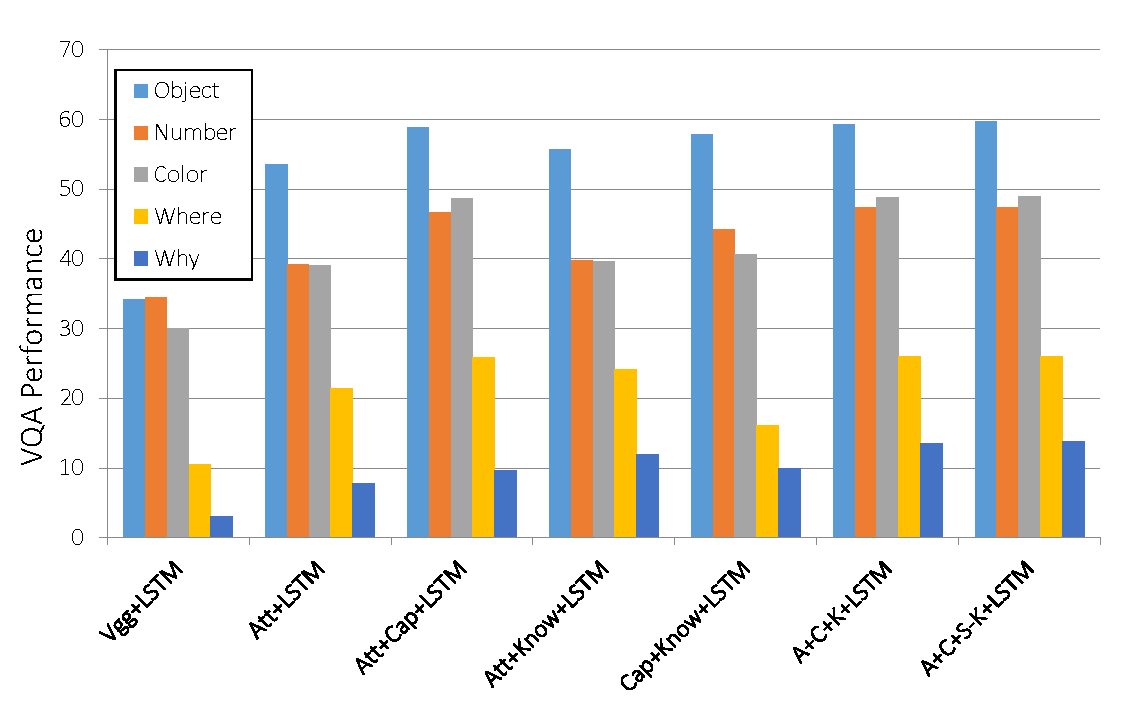
\includegraphics[width=0.9\linewidth]{img/question_cat.pdf}
\end{center}
\vspace{-13pt}
   \caption{Performance on five question categories for different models.}
%
\label{performance_trend}
\end{figure}

Figure~\ref{performance_trend} relates the performance of the various models on five categories of questions. The `object' category is the average of the accuracy of question types starting with `what kind/type/sport/animal/brand...', while the `number' and `color' category corresponds to the question type `how many' and `what color'. The performance comparison across categories is of particular interest here because answering different classes of questions requires different amounts of external knowledge.  The 'Where' questions, for instance, require knowledge of potential locations, and 'Why' questions typically require general knowledge about people's motivation. 'Number' and 'Color' questions, in contrast, can be answered directly. The results show that for 'Why' questions, adding the KB improves performance by more than $50\%$ (Att-LSTM achieves $7.77\%$ while Att+Know-LSTM achieves $11.88\%$), and that the combined A+C+K-LSTM achieves $13.53\%$. We further improve it to $13.76\%$ by using the question-guided knowledge selected model A+C+S-K-LSTM. Compared with the Att-LSTM model, the performance gain of the Cap+Know-LSTM model mainly come from the `why' and `where' started questions. This means that the external knowledge we employed in the model provide useful information to answer such questions. The figure \ref{img:example} shows an real example produced by our model. More questions that require common-sense knowledge to answer can be found in the supplementary materials.

\begin{table}[t!]
\centering
\resizebox{\linewidth}{!}{
 \begin{tabular}{lclccccc}
  \Xhline{2\arrayrulewidth}
  \multicolumn{1}{c}{}         & Our-Baseline &  & \multicolumn{5}{c}{Our Proposal}                                          \\ \cline{2-2} \cline{4-8}
  \multicolumn{1}{c}{Question} & VggNet       &  & Att              & Att+Cap          & Att+Know         & A+C+K            &A+C+S-K\\
  \multicolumn{1}{c}{Type}     & +            &  & +                & +                & +                & +                &+\\
  \multicolumn{1}{c}{}         & LSTM         &  & LSTM             & LSTM             & LSTM             & LSTM             &LSTM\\ \hline
  what is                      & 21.41        &  & 34.63            & 42.21            & 37.11            & \textbf{42.52}   &42.51\\
  what colour                  & 29.96        &  & 39.07            & 48.65            & 39.68            & 48.86            &\textbf{48.89}\\
  what kind                    & 24.15        &  & 41.22            & 47.93            & 46.16            & \textbf{48.05}   & 48.02 \\
  what are                     & 23.05        &  & 38.87            & 47.13            & 41.13            & 47.21            & \textbf{47.27} \\
  what type                    & 26.36        &  & 41.71            & 47.98            & 44.91            & 48.11            & \textbf{48.14} \\
  is the                       & 71.49        &  & 73.22            & 74.63            & 74.40            & \textbf{74.70}   & \textbf{74.70} \\
  is this                      & 73.00        &  & 75.26            & 76.08            & \textbf{76.56}   & 76.14            & 76.17 \\
  how many                     & 34.42        &  & 39.14            & 46.61            & 39.78            & \textbf{47.38}   & \textbf{47.38} \\
  are                          & 73.51        &  & 75.14            & 76.01            & 75.75            & 76.14            & \textbf{76.15} \\
  does                         & 76.51        &  & 76.71            & 78.07            & 76.55            & \textbf{78.11}   & \textbf{78.11} \\
  where                        & 10.54        &  & 21.42            & 25.92            & 24.13            & \textbf{26.00}   & 25.96 \\
  is there                     & 86.66        &  & 87.10            & 86.82            & 85.87            & 87.01            & \textbf{87.33} \\
  why                          & 3.04         &  & 7.77             & 9.63             & 11.88            & 13.53            & \textbf{13.76}  \\
  which                        & 31.28        &  & 36.60            & \textbf{39.55}   & 37.71            & 38.70            & 38.83 \\
  do                           & 76.44        &  & 75.76            & 78.18            & 75.25            & 78.42            & \textbf{78.44} \\
  what does                    & 15.45        &  & 19.33            & 21.80            & 19.50            & 22.16            & \textbf{22.71} \\
  what time                    & 13.11        &  & 15.34            & 15.44            & \textbf{15.47}   & 15.34            & 15.17 \\
  who                          & 17.07        &  & 22.56            & 25.71            & 21.23            & 25.74            & \textbf{25.97} \\
  what sport                   & 65.65        &  & 91.02            & 93.96            & 90.86            & \textbf{94.20}   & 94.18 \\
  what animal                  & 27.77        &  & 61.39            & 70.65            & 63.91            & 71.70            & \textbf{72.33} \\
  what brand                   & 26.73        &  & 32.25            & 33.78            & 32.44            & 34.60            & \textbf{35.68} \\
  others                       & 44.37        &  & 50.23            & 53.29            & 52.11            & 53.45            & \textbf{53.53}     \\ \hline
  Overall                      & 44.93        &  & 51.60            & 55.04            & 53.79            & 55.96            & \textbf{56.17} \\ \Xhline{2\arrayrulewidth}
 \end{tabular}}
\vspace{1pt}
\caption{Results on the open-answer task for various question types on VQA validation set. All results are in terms of the evaluation metric from the VQA evaluation tools. The overall accuracy for the model of \textbf{VggNet+ft+LSTM} and \textbf{Cap+Know+LSTM} is 50.01 and 52.31 respectively. Detailed results of different question types for these two models are not shown in the table due to the limited space.}
\vspace{-12pt}
\label{tab:COCO_Results}
\end{table}

We have also tested on the VQA test-dev and test-standard consisting of 60,864 and 244,302 questions (for which ground truth answers are not published) using our final A+C+S-K-LSTM model, and evaluated them on the VQA evaluation server. Table \ref{tab:server_results_2} shows the server reported results. The results on the Test-dev can be found in the supplementary material.

Antol \etal \cite{antol2015vqa} provide several results for this dataset. In each case they encode the image with the final hidden layer from VggNet, and questions and captions are encoded using a BOW representation. A softmax neural network classifier with 2 hidden layers and 1000 hidden units (dropout 0.5) in each layer with tanh non-linearity is then trained, the output space of which is the 1000 most frequent answers in the training set. They also provide an LSTM model followed by a softmax layer to generate the answer. Two version of this approach are used, one which is given only the question and the image, and one which is given only the question (see~\cite{antol2015vqa} for details). %
Our final model outperforms all the listed approaches according to the overall accuracy. Figure \ref{results_examples} provides some indicative results. More results can be found in the supplementary material.

%

